\part{Annexes}
    \chapter{l'API sencrop}
  Sencrop met à la disposition de ses utilisateurs une API rest permettant de faire des requêtes et de récupérer les informations. Il utilise le protocole https qui garantit la confidentialité des échanges entre l’utilisateur et l’API. Un utilisateur doit avoir un jeton(token)  pour pouvoir communiquer avec les serveurs de Sencrop par le mécanisme de HTTP Bearer.Il est possible d’obtenir un jeton  via 2 flux distincts : le flux SMS ou le flux de module.
  \begin{itemize}
      \item Le flux vous permet de créer directement des jetons. La condition préalable est que l'utilisateur doit avoir activé au moins un de ses modules(station météo) sur son application Sencrop.
      \item Flux SMS il est également possible d’obtenir un jeton auprès des utilisateurs de Sencrop en leur envoyant un SMS avec un code de validation qui  permet de demander à un 'utilisateur l'autorisation d'accéder à ses données.
  \end{itemize}

    \begin{figure}[!h]
        \centering
        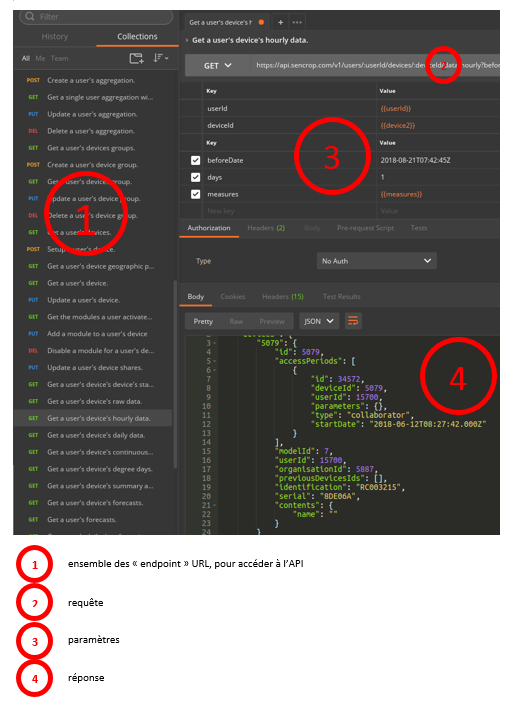
\includegraphics[height=.5\textheight]{images/api_image.jpg}
    \end{figure}
    
    
    \chapter{Documentation sur les données fournis par les stations météo}
    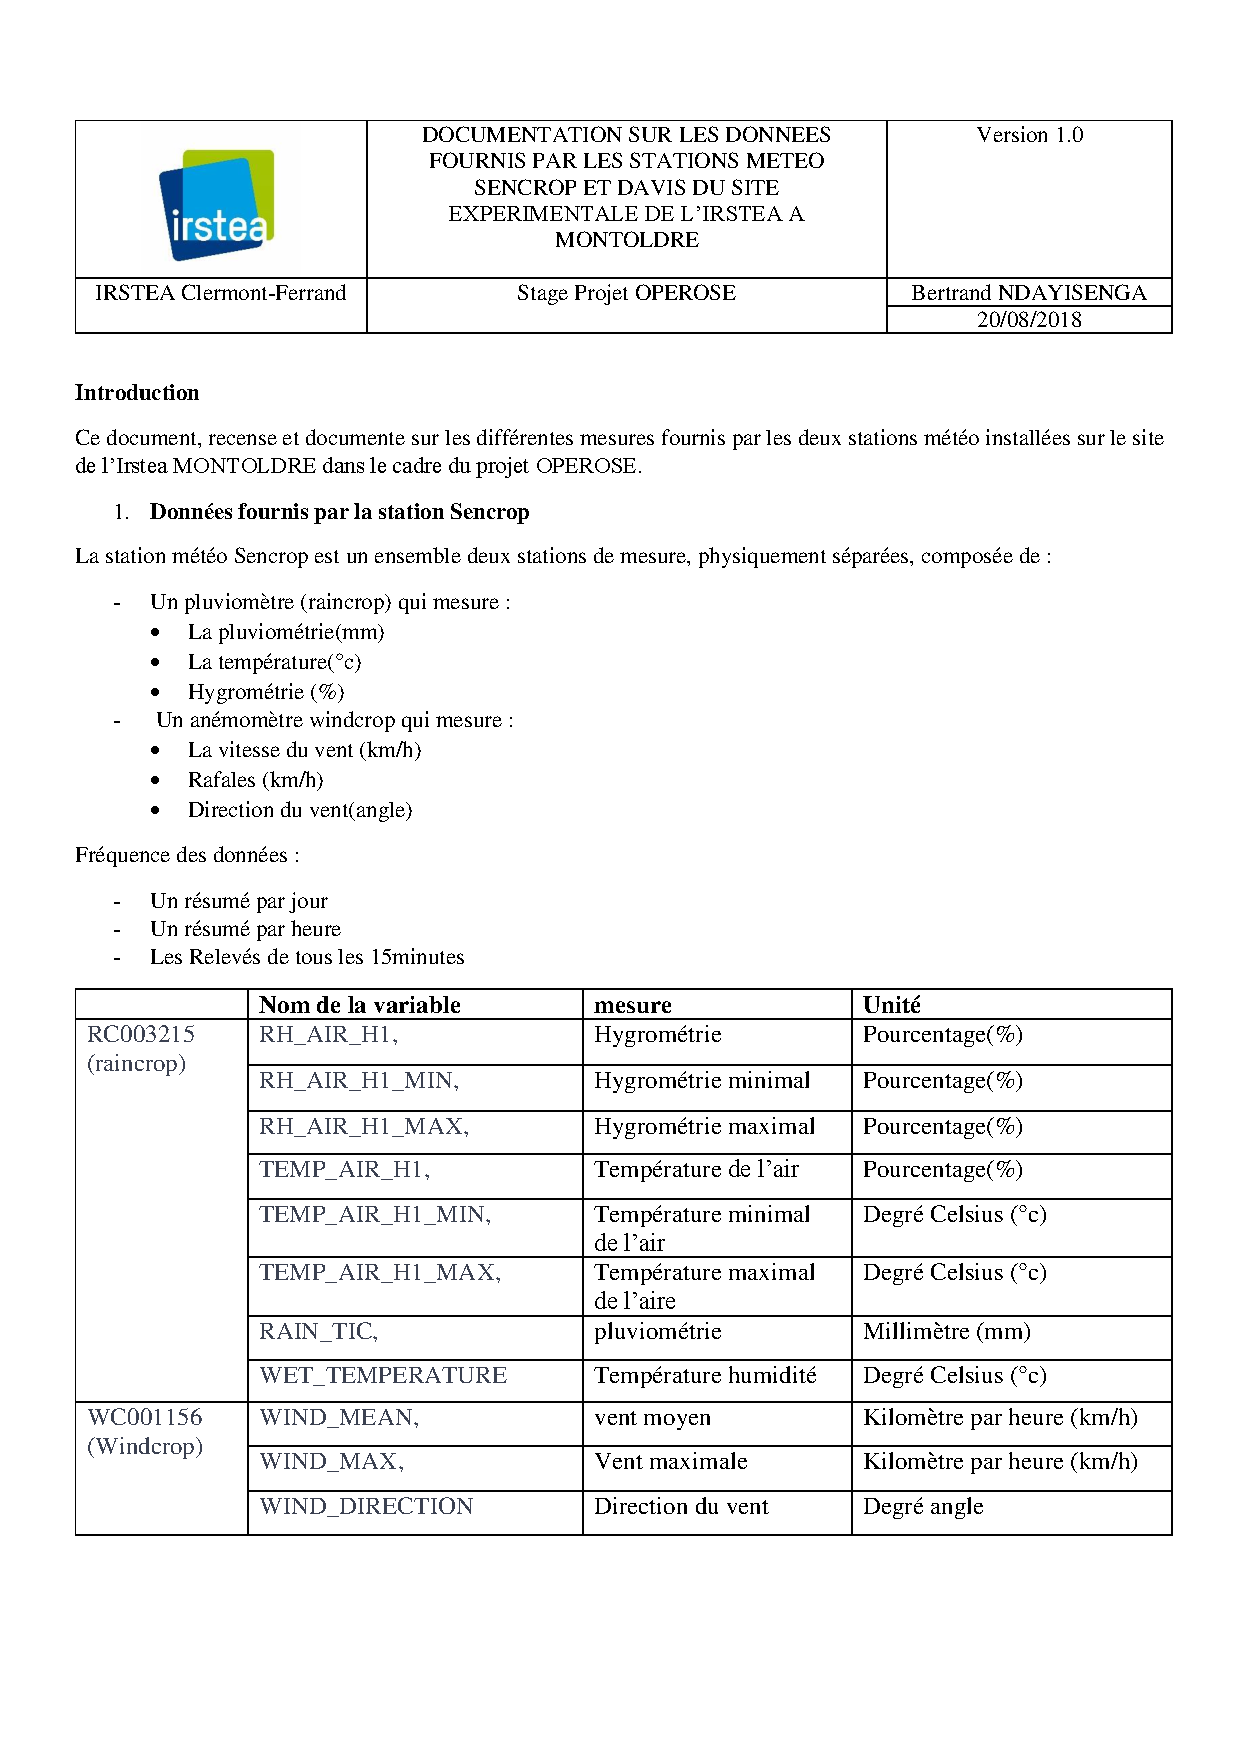
\includepdf[pages={1-3}]{pdfFiles/documentations.pdf}